\documentclass{beamer}

\usepackage[utf8]{inputenc}
\usepackage{braket}
\usepackage{parskip}
\usepackage{verbatim}
\usepackage{natbib}

\begin{filecontents}{\jobname.bib}
    @article {[1],
	  author = {Platzman, P. M. and Dykman, M. I.},
	  title = {Quantum Computing with Electrons Floating on Liquid Helium},
	  volume = {284},
	  number = {5422},
	  pages = {1967--1969},
	  year = {1999},
	  doi = {10.1126/science.284.5422.1967},
	  publisher = {American Association for the Advancement of Science},
	  issn = {0036-8075},
	  URL = {https://science.sciencemag.org/content/284/5422/1967},
	  eprint = {https://science.sciencemag.org/content/284/5422/1967.full.pdf},
	  journal = {Science}
    }

    @article{[2],
    title = {Qubits with electrons on liquid helium},
    author = {Dykman, M. I. and Platzman, P. M. and Seddighrad, P.},
    journal = {Phys. Rev. B},
    volume = {67},
    issue = {15},
    pages = {155402},
    numpages = {15},
    year = {2003},
    month = {Apr},
    publisher = {American Physical Society},
    doi = {10.1103/PhysRevB.67.155402},
    url = {https://link.aps.org/doi/10.1103/PhysRevB.67.155402}
    }

    @article{[3],
    title = {Spin-based quantum computing using electrons on liquid helium},
    author = {Lyon, S. A.},
    journal = {Phys. Rev. A},
    volume = {74},
    issue = {5},
    pages = {052338},
    numpages = {6},
    year = {2006},
    month = {Nov},
    publisher = {American Physical Society},
    doi = {10.1103/PhysRevA.74.052338},
    url = {https://link.aps.org/doi/10.1103/PhysRevA.74.052338}
    }

    @article{4,
    title = {Proposal for Manipulating and Detecting Spin and Orbital States of Trapped Electrons on Helium Using Cavity Quantum Electrodynamics},
    author = {Schuster, D. I. and Fragner, A. and Dykman, M. I. and Lyon, S. A. and Schoelkopf, R. J.},
    journal = {Phys. Rev. Lett.},
    volume = {105},
    issue = {4},
    pages = {040503},
    numpages = {4},
    year = {2010},
    month = {Jul},
    publisher = {American Physical Society},
    doi = {10.1103/PhysRevLett.105.040503},
    url = {https://link.aps.org/doi/10.1103/PhysRevLett.105.040503}
    }
\end{filecontents}

\bibliographystyle{abbrv}
%\renewcommand\bibfont{\scriptsize}

\usefonttheme{serif}

\title{Quantum Computing \\ with Electrons on Helium}
\subtitle{\vspace*{5mm}\large{Physkiss-1}}
\author{\vspace*{-1cm}Sanskriti Chitransh}
\date{\vskip\small{3rd June, 2020}}

\setbeamercolor{background canvas}{bg=pink!50}
\setbeamercolor{title}{fg=gray!140}
\setbeamercolor{author}{fg=gray!140}
\setbeamercolor{date}{fg=gray!140}
\setbeamercolor{normal text}{fg=gray!140}
\setbeamercolor{frame title}{fg=gray!140}
\setbeamercolor{enumerate item}{fg=gray!140}
\setbeamercolor{itemize item}{fg=gray!140}

\setbeamercolor*{bibliography entry title}{fg=gray!140}
\setbeamercolor*{bibliography entry author}{fg=gray!140}
\setbeamercolor*{bibliography entry location}{fg=gray!140}
\setbeamercolor*{bibliography entry note}{fg=gray!140}

\setbeamerfont{title}{series=\bfseries,parent=structure}
\setbeamerfont{author}{series=\bfseries,parent=structure}
\setbeamerfont{date}{series=\bfseries,parent=structure}

\setbeamersize{text margin left=10mm,text margin right=10mm} 

\setbeamertemplate{bibliography item}{}
\setbeamertemplate{frametitle continuation}[from second]
\setbeamertemplate{frametitle}{\color{gray!140}\rmfamily\bfseries\vspace{0.5cm}\insertframetitle\vskip-2pt\hrulefill}



\begin{document}

\usebeamercolor[fg]{normal text}

\maketitle

\section{Introduction}
\begin{frame}[t]{Format of the talk}
    \begin{enumerate}
        \item DiVincenzo criteria for realizing physical quantum computation
        \item Experimental setup
        \item Single qubit and multiple qubit arrangements
        \item Decay, decoherence and relevant timescales
        \item Quantum gates and readout
    \end{enumerate}
\end{frame}

\section{DiVincenzo Criteria}
\begin{frame}[t]{DiVincenzo Criteria}
    Experimental conditions necessary for quantum computation:
    \begin{enumerate}
       \item A scalable physical system with well characterized qubits
        \item The ability to initialize the state of the qubits to a “ground state”
        \item Long relevant decoherence times
        \item A “universal” set of quantum gates
        \item  A qubit-specific measurement capability
    \end{enumerate}
\end{frame}

\section{Experimental setup}
\begin{frame}[t]{Experimental setup}
    \begin{itemize}
        \item Single electron trapped on a bulk liquid Helium film at $T < 0.1 K$
        \item Image potential seen by electron is $\mathbf{V = \Lambda e^2/z}$
    \end{itemize}
    \centering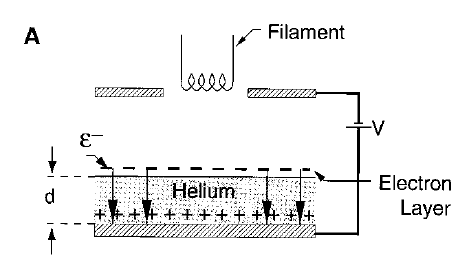
\includegraphics[height=4cm]{images/setup.png}
\end{frame}

\section{Single qubit}
\begin{frame}{Qubit}
    \begin{columns}
        \begin{column}{0.48\textwidth}
            \begin{itemize}
                \item Electron $z$ motion described by $1-D$ Hydrogenic potential:
                    $$\mathbf{E_m = -R/m^2}$$
                for the $m$'th state with Rydberg energy $R\cong 8K$.
                \item Rabi frequency $\sim GHz$
            \end{itemize}
        \end{column}
        \begin{column}{0.48\textwidth}  %%<--- here
            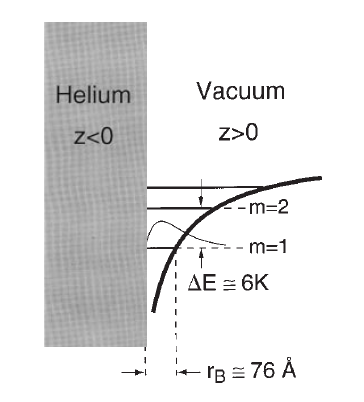
\includegraphics[height=5cm]{images/single qubit.png}
        \end{column}
    \end{columns}
\end{frame}

\section{multi qubit}
\begin{frame}[t]{Multiple qubits}
    \begin{itemize}
        \item Substrate with patterned electrodes for lateral "in-plane" confinement
        \item In-plane quantum energy levels created, harmonic oscillations at $\mathbf{\omega_{\parallel}/2\pi \approx 10-20 GHz}$ for $\mathcal{E}_{\perp}= 500 V/cm$ and $h=0.5\mu m$
        \item Qubit characterization $\mathbf{\equiv \ket{i, v, m_v}}$
    \end{itemize}
    \centering\includegraphics[height=3.5cm]{images/multi qubit.png}
\end{frame}

\section{}
\begin{frame}[t]{Relaxation: Ripplons}
    \begin{itemize}
        \item Ripplons are vibrations of the liquid He surface 
        \item Electron-ripplon coupling takes the form: $$\mathbf{H_{i}^{(1)} = \sum\limits_{q}\xi_{q}e^{i(q \cdot r)}\hat{V}_q}$$
        The quadratic term is: $$\mathbf{H^{(2)}_i = \sum\limits_{q_1,q_2}\xi_{q_1}\xi_{q_2}exp[i(q_1+q_2)r]\hat{V}_{q_1,q_2}}$$
    \end{itemize}
\end{frame}

\section{Relaxation: One-Ripplon Processes}
\begin{frame}[t]{Relaxation: One-ripplon processes}
    \begin{itemize}
        \item Decay of $\ket{2,0,0}$ does not require transition to $\ket{1,0,0}$;  $\ket{2,0,0}\rightarrow\ket{1,v,m_v}$ transitions are possible        
        \item Energy conservation in a transition requires too large ripplon momentum for an electron to accommodate
        \item One-ripplon decay rate is calculated from the coupling Hamiltonian and is exponentially small for $\omega_{\parallel}\sim 20 GHz$
        \item Sufficiently suppressed by strong in-plane confinement
    \end{itemize}
\end{frame}

\section{}
\begin{frame}[t]{Relaxation: Two-ripplon processes}
    \begin{itemize} 
    \item Two ripplons with large wave vectors $\mathbf{q_1,q_2}$ emitted 
    \item Propagate in opposite directions at nearly the same frequencies 
    \item For minimal electron energy change $\hbar\omega_{\parallel}$ ripplon frequencies $\sim \omega_{\parallel}$ 
    %\item $\mathbf{T_1 \sim  1000\mu s}$
    \end{itemize}
\end{frame}

\section{}
\begin{frame}[t]{Dephasing}
    Definition: diffusion of phase difference between $\ket{2,0,0}$ and $\ket{1,0,0}$  by quasielastic scattering of thermal excitations
    \begin{itemize}
         \item Primary source is coupling to ripplons
         \item Density of states for thermally excited ripplons is high even at low temperatures
         \item Dephasing rate depends on both frequency of singly coupled ripplons and $k_B T/\hbar$
         %\item $\mathbf{T_2 \sim 100\mu s}$ 
    \end{itemize}
\end{frame}

\section{}
\begin{frame}[t]{Single-qubit gates }
    \begin{itemize}
        \item State changed by application of microwave frequencies
    \end{itemize}
\end{frame}

\section{}
\begin{frame}[t]{Two-qubit gates}
    \begin{itemize}
        \item Resonant frequencies controlled by patterned electrode voltage
        \item Electron-electron Coulomb interaction:
        $$\mathbf{V_c (z_1,z_2) \cong \frac{e^2}{d^3}(z_1 z_2)}$$
    \end{itemize}
    \begin{center}
        \includegraphics[height=3cm]{multi qubit.png}
    \end{center}
\end{frame}

\section{}
\begin{frame}[t]{Qubit readout}
    \begin{itemize}
        \item Reverse field (just strong enough) applied to capacitor
        \item Electron sees potential as shown, tunnelling strength depends on strength of field
        \item Arrival time of electrons leaving the He surface strong function of $\mathbf{m}$
    \end{itemize}
    \begin{center}
        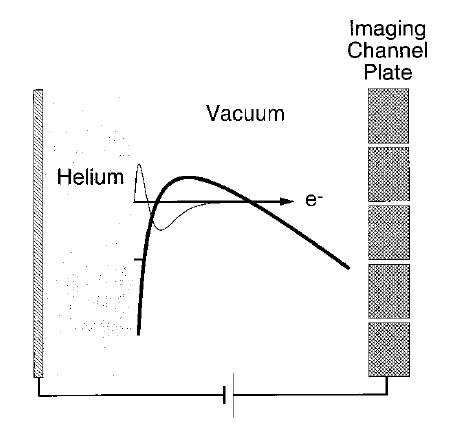
\includegraphics[height=4cm]{images/readout.png}
    \end{center}
\end{frame}


\begin{comment}
\section{}
\begin{frame}[t]{David's paper}
    \begin{itemize}
        \item  
    \end{itemize}
\end{frame}
\end{comment}

\section{}
\begin{frame}[t]{References}
    Images from \cite{[2]}; rest from \cite{[2]} and \cite{[1]}.
   
    \bibliography{\jobname}
\end{frame}

\section{}
%\setbeamertemplate{footline}{and I love you $\heartsuit$}
\begin{frame}{}
    \usebeamercolor[fg]{normal text}
    \begin{center}
        \Large{\textbf{Thank you!}}
    \end{center}
 % these braces make the change local to the single frame
        
\end{frame}


\end{document}
